\section{Using a Virtual Machine}

Just like a tree-walking interpreter, a virtual machine presents a method of implementing an interpreter for a programming language.
However, the way a virtual machine operates fundamentally differs from the one which the tree-walking interpreter uses.
For rush, we have implemented a virtual machine backend in order to compare it to the previously displayed tree-walking interpreter.

\subsection{Defining a Virtual Machine}

Often, one might encounter the term \emph{virtual machine} when talking about emulating an existing type of computer using a software system.
This emulation often includes simulating additional devices like the computer's display or its disk.
In this context however, a \emph{virtual machine} is a software entity which emulates how a computer interprets instructions.
Just like a real computer, a virtual machine executes low-level instructions directly.

Since a physical processor and a virtual machine share some fundamental traits,
the architecture of a virtual machine is often a slight deviation from the von Neumann architecture.
The von Neumann architecture was first introduced by John Neumann in the year 1945.
Von Neumann originally presented a design which allows implementing a computer using relatively few components.
A von Neumann computer usually contains components like an \emph{ALU}\footnote{Short for \enquote{arithmetic logic unit}}, multiple registers, a control unit, memory, and basic IO \cite[p.~172]{Ledin2020-yp}.
The ALU is designed in order to perform logical and mathematical operations as fast as possible.
However, in order to keep its implementation simple, it lacks the ability to fetch instructions from memory directly.
Therefore, a von Neumann processor contains a control unit which manages the \emph{fetch-decode-execute} cycle.
This cycle is a simplification of the steps a processor performs in order to execute instructions.

\begin{itemize}
	\item \textbf(Fetch): The processor's control unit loads the next instruction from the adequate memory location.
	      The value of the next instruction is then placed into the processor's internal instruction register.
	\item \textbf(Decode):
	      The processor's control unit examines the fetched instruction in order to determine if additional steps must be taken during instruction execution.
	      Such steps may involve accessing additional registers or memory locations.
	\item \textbf(Execute):
	      The control unit dispatches the instruction to a specialized component of the processor.
	      The target component is often dependent on the type of instruction since each processor component is optimized with one specific type of instruction in mind.
	      For instance, the control unit may invoke the ALU in order to perform a mathematical operation.
\end{itemize}

A computer's processor performs this fetch-decode-execute cycle repeatedly from the moment it is powered on until the point in time where it is powered down again.
For relatively simple processors, each cycle is executed in an isolated manner because instructions are executed in a sequential order.
This means that the execution of the instruction $i$ is delayed until execution of $i - 1$ has completed \cite[pp.~208-209]{Ledin2020-yp}.

For most virtual machines, executing the input instructions in sequential order is often the simplest solution.
Often, a virtual machine implements a method of instruction execution similar to the fetch-decode-execute cycle.
It is now apparent that a virtual machine is unable to traverse the AST directly and therefore relies on a sequence of instructions as its input.
Although the von Neumann architecture is relatively simple, one must not always adopt it when choosing how to implement a virtual machine.
Since virtual machines are purely abstract constructs, meaning that they are implemented using software, design constrains are usually kept to a minimum.
A large benefit of virtual machines is that the source program runs significantly faster at runtime.
Therefore, implementing a programming language to run on a virtual machine is often a reasonable idea.
A reason for this speedup is that tree-traversal involves a lot of overhead which is omitted when interpreting instructions directly.

\TSListing[first line=5, caption={A Recursive rush Program}, label={lst:rush_vm_faster}, float=H]{listings/vm_faster.rush}
\noindent
\begin{figure}[h]
	\begin{minipage}{.7\textwidth}
		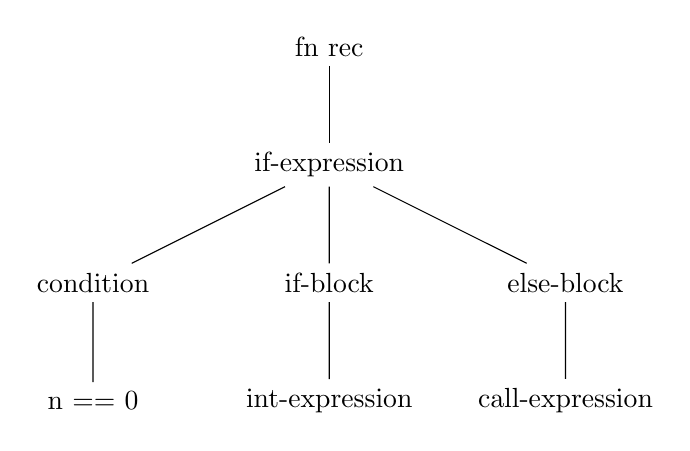
\begin{tikzpicture}[
				tlabel/.style={pos=0.4,right=-1pt,font=\footnotesize\color{red!70!black}},
			]
			\node{fn rec}
			child { node {if-expression}
					child { node {condition} child {node {n == 0}} }
					child [missing]
					child { node {if-block} child {node {int-expression}} }
					child [missing]
					child { node {else-block} child{node{call-expression}} }
				};
		\end{tikzpicture}
	\end{minipage}%
	\begin{minipage}{.3\textwidth}
		\TSListing[raw=true, frame=none]{listings/vm_faster_instructions.txt}
	\end{minipage}
	\caption{Syntax Tree and VM instructions of a Recursive rush Program}
	\label{fig:tree_vs_vm}
\end{figure}

Figure \ref{fig:tree_vs_vm} displays a heavily simplified syntax tree and rush VM instructions representing the recursive program from above.
The root node of the syntax tree represents the \texttt{rec} function.
Since the function only contains a single expression, the if-expression node follows as the only child of the root node.
The if-expression contains a condition, an if-branch, and an else-branch.
Since the function should not call itself again if \texttt{n} is equal to 0, the if-block returns 0.
The else-block however calls the \texttt{rec} function recursively.
If the above program is executed, the tree-walking interpreter would have to traverse the entire tree of the \texttt{rec} function every time it is called.
Since \texttt{rec} is a recursive function, the tree-walking interpreter would have to traverse it $n$ times.
In this example, the syntax tree of the program is relatively simple.
However, the syntax tree of a more complex program will also contain more complexity.
Since loops and recursive functions execute the code in their bodies repeatedly, the tree traversal of the body presents an inefficiency.
Here, the inefficiency solely lies in the repeated tree-traversal, not in the repetition introduced by an iterative or recursive algorithm.
In order to improve efficiency, an algorithm could traverse the tree once, saving its semantic meaning in the process.
Then, the semantic meaning of the previously traversed tree could be interpreted repeatedly without this much overhead.

% TODO: draw final conclusions
Virtual machines can often mitigate this issue by interpreting instructions directly.

\subsection{Registers and Stack-Based Machines}

Often, physical processors use \emph{registers} in order to make larger computations possible.
Registers are a limited set of very fast, low capacity storage units.
On modern architectures, like \emph{x86\_64}, each general-purpose register is able to hold as much as 64 bits of information.
However, there is always only a limited amount of registers available since.
Therefore, programs often only utilize registers for storing temporary values, such as intermediate results of a large computation.
The main alternative to using registers is a stack-based design.
A popular example for a stack-based virtual machine is \emph{WebAssembly}.
Stack-based machines are often significantly easier to program since register allocation can be completely omitted.

For compiler writers, register allocation is often a demanding task
% TODO: link to the correct chapter
However, this problem is described in more detail in the later chapters.
A stack-based machine is often significantly simpler since registers are omitted entirely.
Therefore, one might chose to implement a stack-based virtual machine in order to minimize complexity of the program.
However, a stack-based layout also introduces several issues on its own.
For instance, register-based machines might regularly outperform stack-based machines.
Furthermore, using the stack usually involves a lot of push or pop instructions which could have otherwise been omitted.

\subsection{The rush Virtual Machine}

\subsection{How the Virtual Machine Executes A rush Program}
\subsection{The Compiler Targeting the Virtual Machine}
